\documentclass[a4paper,addpoints, 12pt]{exam}
%\documentclass[answers,14pt]{exam}
\unframedsolutions

\usepackage{pdfpages}

\usepackage{array,amsmath,fancybox,amsfonts,graphicx,amsthm,amssymb,wasysym}
\usepackage{latexsym,slashed,subfigure,calc}
\usepackage[spanish]{babel}
\usepackage[utf8]{inputenc}
%\usepackage{fancyhdr,float,hyperref}
%\usepackage{lettrine}


%entorno para química: texto y math mode
	%\newcommand*\chem[1]{\textup{#1}}
	\newcommand*\chem[1]{\ensuremath{\mathrm{#1}}}

%tamaños fuentes extra: 8,9,14,17,20
	\usepackage{extsizes}

%display style in long fractions
	\newcommand\ddfrac[2]{\frac{\displaystyle #1}{\displaystyle #2}}

%tabla generada
%	\usepackage[table,xcdraw]{xcolor}

%lewis y química
\usepackage{chemformula,elements}
%chemformula, provides \ch{} with the !(<below>)(<formula>) syntax and \chlewis;
%elements, provides \elconf and \writeelconf.
%ex:
%\ch{
%  !(\elconf{Li})( "\chlewis{180.}{Li}" ) +
%  !(\elconf{F})( "\chlewis{0.90:180:270:}{F}" )
%   ->
%  !(\writeelconf{2})( Li+ ) +
%  !(\writeelconf{2,2+6})( "\chlewis{0:90:180:270:}{F}" {}- )
%}

%multicol
\usepackage{multicol}
  

%símbolo bonito para qed
\usepackage{amsthm}
	%\newcommand{\mc}[3]{\multicolumn{#1}{#2}{#3}}
\newcommand{\halmos}{\vspace*{-5mm}
	
					\begin{flushright}
						\rule{1mm}{2.5mm} 
					\end{flushright}
					\vspace*{-4mm}
						
					  }
\renewcommand{\qed}{\halmos}

 
%página blanco
%\usepackage{afterpage}
%uso \afterpage{\blankpage}

\newcommand\blankpage{%
    \null
    \thispagestyle{empty}%
    \addtocounter{page}{0}%
    \newpage}


 %caja bonita
  \usepackage[many]{tcolorbox}
\definecolor{titlebg}{RGB}{80,100,72}
\newtcolorbox{learn}{
  breakable,
  enhanced,
  arc=0pt,
  outer arc=0pt,
  colframe=titlebg,
  colback=titlebg!7,
  overlay unbroken and first={
    \node[
      draw=titlebg,
      fill=titlebg,
      rotate=270,
      anchor=north west,
      text=white,
      font=\bfseries
    ]
    at (frame.north west)  
    {DATOS};
  }
}


\newtcolorbox{problemas}{
  breakable,
  enhanced,
  arc=0pt,
  outer arc=0pt,
  colframe=titlebg,
  colback=titlebg!7,
  overlay unbroken and first={
    \node[
      draw=titlebg,
      fill=titlebg,
      rotate=270,
      anchor=north west,
      text=white,
      font=
    ]
    at (frame.north west)  
    {AVISO};
  }
}
	
\usepackage{anysize}
	%\marginsize{left}{right}{top}{bottom}
    \marginsize{1.3cm}{1cm}{.4cm}{.75cm}

\usepackage{sidecap}
\usepackage{mwe,float,afterpage}

%redefiniciones
\pointpoints{punto}{puntos}
\bonuspointpoints{punto}{puntos}
\hqword{Pregunta} %substitutes text for \Question"
%\vpgword{Pág.}%substitutestext for \Page"
\hpword{Máx.}%substitutes text for \Points"
\hsword{Nota}%substitutes text for \Score"
\htword{Total}%substitutes text for \Total:"

\chqword{Pregunta}
\chpword{Máx.}
\chsword{Nota}
\chtword{Total}
\chbpword{Puntos \textit{bonus}}

\renewcommand{\solutiontitle}{\noindent\textbf{Solución:}\par\noindent}


%fuentes
	%\usepackage[T1]{fontenc}
	%\usepackage{fourier}

	\usepackage[T1]{fontenc}
	\usepackage{librebaskerville}


\usepackage{graphicx,graphics}
\usepackage{color}
	%	\colorgrids %grids con color
	%	\definecolor{GridColor}{gray}{0.8}
		%grid
%			\setlength{\gridsize}{5mm}
%   			 \setlength{\gridlinewidth}{0.1pt}

%fracciones en texto más elaboradas
	\usepackage{xfrac}

%mejora en la exposición de guarismos
	\usepackage{numprint}
 
%caption
\usepackage[font=small,labelfont=bf,
labelsep=endash]{caption}
	
%soluciones sombreadas	
\shadedsolutions


\checkboxchar{$\Box$}
\checkedchar{$\blacksquare$}

\usepackage{everypage,draftwatermark} %Marca de agua
\SetWatermarkText{\parbox{\textwidth}{\centering Xtra}}
\SetWatermarkScale{2.5}
\SetWatermarkLightness{0.9}



%
%\usepackage{background}
%\backgroundsetup{
%scale=1.5,
%angle=180,
%opacity=.05,
%color=black,
%contents={
%\includegraphics[scale=1]{unicorn.jpg}}}



%espacios extra
%\extrawidth{3ex}
%%\extrafootheight{.75in}
%\extraheadheight{1in}

%cabecera
\header{} {}  {}   
           
%pie de página

   %enumera en todas menos en la primera
   %\runningfootrule

   %enumera en todas
   %\footrule
   %\footer{}{Página \thepage\ de \numpages}{}
%   \footer{}
%	{Página \thepage\ de \numpages}
%	{\iflastpage{{\footnotesize \textit{Fin del examen}}}{{\footnotesize \textit{Da la vuelta a la hoja}\ldots}}}


%indents 
\renewcommand{\questionlabel}{\makebox[1cm][l]{\thequestion}}
\renewcommand\partlabel{\makebox[1cm][l]{\alph{partno})}}

\renewcommand{\questionshook}{%
  \setlength{\leftmargin}{0pt}%
  \setlength{\labelsep}{0pt}
  \setlength{\labelwidth}{0pt}%
}

\renewcommand{\partshook}{%
  \setlength{\leftmargin}{1pt}%
  \setlength{\labelsep}{-12pt}
  \setlength{\labelwidth}{4ex}%
  \def\makelabel##1{##1}%
}


  
\begin{document}
	\begin{coverpages}
%portada
\pagenumbering{gobble}


%formato de preguntas
\qformat{\textbf{Pregunta \thequestion}\hfill} 
\boxedpoints



\fbox{\parbox{0.945\linewidth}{\textbf{Nombre y apellidos}:\vspace*{20mm}}}
\vspace*{\fill}

\begin{learn}
{$\triangleright\; M(\chem{O})\simeq16\;g\,mol^{-1}$\newline
$\triangleright\; M(\chem{C})\simeq12\;g\,mol^{-1},$\newline
$\triangleright\; M(\chem{N})\simeq14\;g\,mol^{-1},$\newline
$\triangleright\; M(\chem{H})\simeq1\;g\,mol^{-1},$\newline
$\triangleright\; M(\chem{Na})\simeq 23\;g\,mol^{-1},$\newline
%$\triangleright\; M(\chem{Cl})\simeq 36\;g\,mol^{-1},$\newline
%$\triangleright\; M(\chem{S})\simeq32\;g\,mol^{-1},$\newline
%$\triangleright\; M(\chem{Mn})\simeq55\;g\,mol^{-1},$\newline
%$\triangleright\; M(\chem{Cu})\simeq64\;g\,mol^{-1},$\newline
$\triangleright\; R\simeq 0.082\;atm\,L\,mol^{-1}\,K^{-1}$
}
\end{learn}	
\end{coverpages}

\newpage
\vspace*{-5ex}

\begin{problemas}{Esta prueba tiene \numquestions\ preguntas y un total de \numpoints\ puntos. Es una  \textit{comunicación}: invoca las leyes en que te basas e \textit{indica brevemente los pasos y razonamientos} que sigues.}
\end{problemas}

\begin{questions}

\question Considera los elementos desconocidos $_{8}\alpha$,\hspace{1ex} $_{37}\beta$,\hspace{1ex} $_{39}\delta$,\hspace{1ex} $_{53}\varepsilon.$ 
    	\begin{parts}
    		\part[1] Describe las propiedades (\textit{enlace, solubilidad, conducción eléctrica y estado físico a temperatura ambiente}) que presentará el compuesto que forman $\delta$ y $\varepsilon$.
    		\part[\half] Justifica la existencia de la molécula $\alpha_2$ e indica el tipo de enlace que se da.
    		\part[\half] Indica los números cuánticos de los electrones de la capa de valencia de $\beta$.		
    	\end{parts}
		\qed

\question El amoniaco reacciona con oxígeno molecular para dar óxido de nitrógeno{\footnotesize(II)} y agua. En un reactor estanco se introducen $200\;g$ de amoniaco y $30$ moles de una mezcla gaseosa cuya fracción molar de dioxígeno es $\chi=0.4$.
    	\begin{parts}
    		\part[2] Determina el reactivo limitante y los gramos de reactivo que sobran.
    		\part[\half] Determina los gramos de óxido de nitrógeno{\footnotesize(II}) que se obtienen si el rendimiento para su producción es del $70\%$.
    	\end{parts}
  	\qed


\question En un reactor se quiere preparar la reacción de peróxido de sodio con agua para producir hidróxido de sodio sólido y oxígeno molecular gaseoso. 
	\begin{parts}
    		\part[2] Determina el volumen teórico de gas producido a partir de una muestra de $10\;g$ de peróxido de sodio si las condiciones finales en el reactor son de $20^\circ C$  y $1.5\;atm$.
    		\part[\half] Al hacer el experimento se encuentra que el volumen real producido es de $780\;cm^3$, ¿cuál es el rendimiento de la reacción para la formación de oxígeno?
    	\end{parts}
\qed


\question Un cañón antiaéreo {\footnotesize BOFORS 80MM} es capaz de disparar en cualquier dirección con una velocidad inicial de $700\;ms^{-1}$. Si los disparos se efectúan con una inclinación de $55^\circ$ respecto del suelo y consideramos despreciables los efectos del rozamiento con el aire:
	\begin{parts}
		\part[\half] Describe el sistema de referencia que usarás para estudiar el proyectil.
		\part[1] Calcula el módulo de su velocidad un segundo después del lanzamiento.
		%$\simeq 690\;ms^{-1}$
		\part[1] Calcula la altura máxima, desde la boca del cañón, que alcanza el proyectil.
		%$\simeq 16.5\;km$
	\end{parts}
	\qed

\vspace{2ex}

\begin{minipage}{.71\textwidth}
\question
\hfill \newline Una caja de masa $m=10\;kg$ está situada sobre una rampa y se encuentra  unida a la pared por una cuerda. La tensión máxima que aguanta la cuerda antes de romperse es de $80\;N$.

	\begin{parts}
		\part[\half]  Representa las fuerzas que actúan en el sistema.
		\vspace{-1ex}
		
		\part[1] Calcula el ángulo máximo que puede formar el suelo con la rampa para que la cuerda no se rompa.
		
	\end{parts}
\end{minipage}\hfill
\begin{minipage}{.27\textwidth}
\vspace{1ex}

	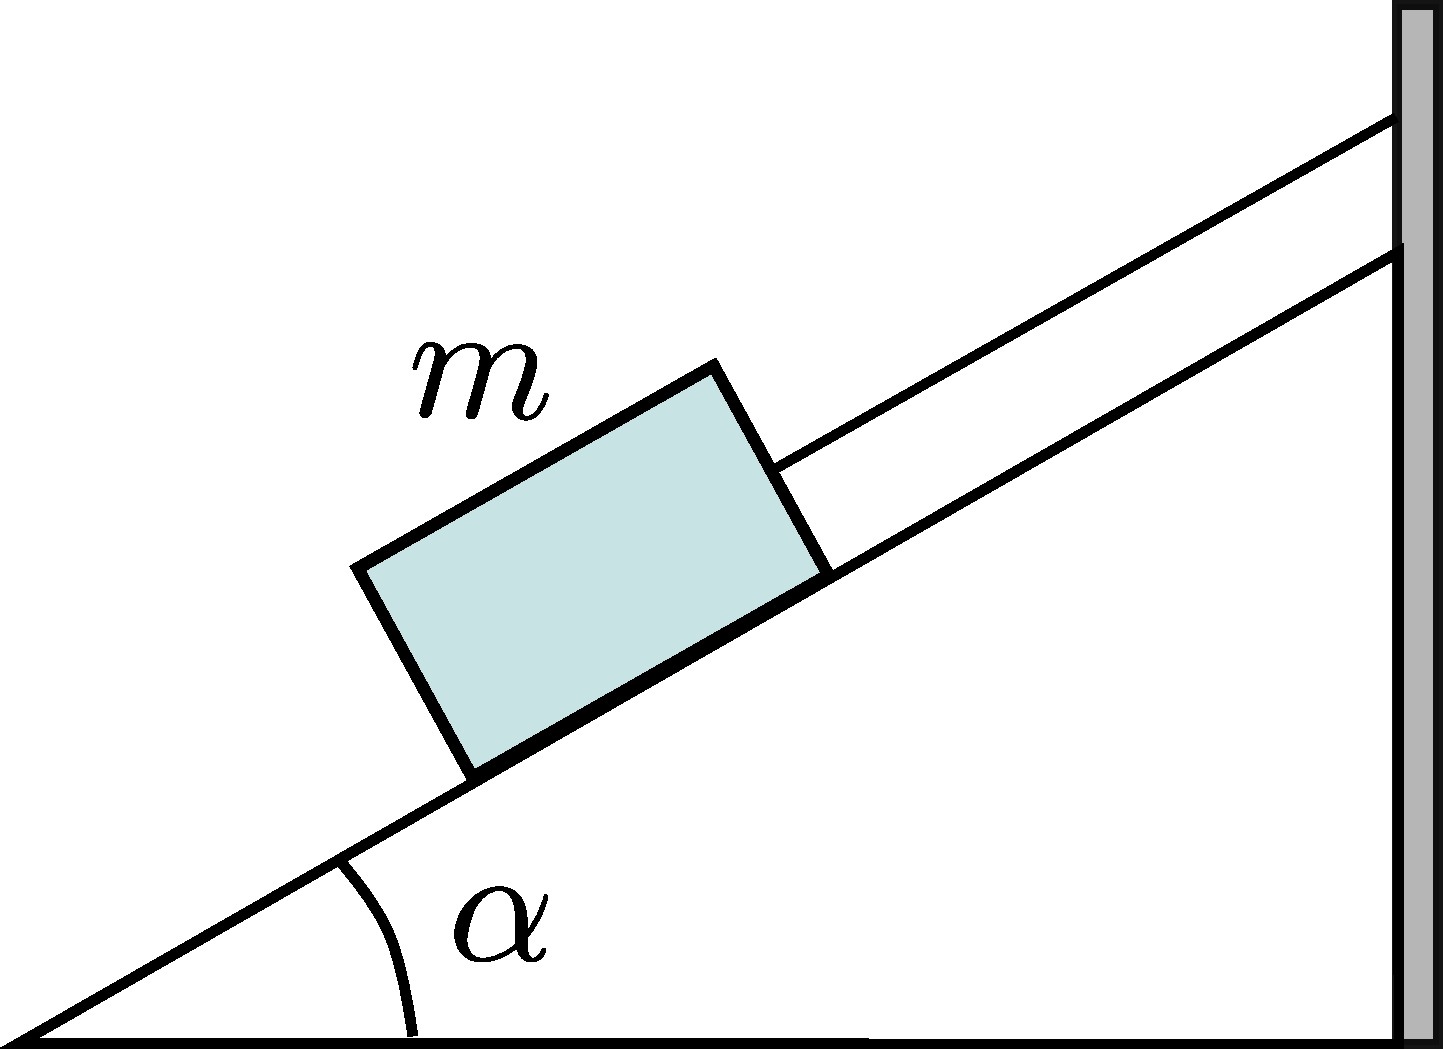
\includegraphics[scale=.18]{rampa.pdf}
	\vspace{1ex}

\end{minipage}
\begin{parts}
\setcounter{partno}{2}
\part[1] Si montamos el sistema con un ángulo un $10\%$ mayor que el ángulo máximo que acabas de calcular, y suponiendo que hay un coeficiente de fricción $\mu=0.1$ con la rampa, ¿cuál es la aceleración del bloque después de rota la cuerda?
%\part[1] Despreciando el rozamiento, ¿cuánto debe valer $\sfrac{M}{m}$ para que un astronauta cualquiera caiga con una aceleración $a$?	
\end{parts}
\qed

\end{questions}	

\newpage

\SetWatermarkText{}
\SetWatermarkScale{2.5}
\SetWatermarkLightness{0.9}


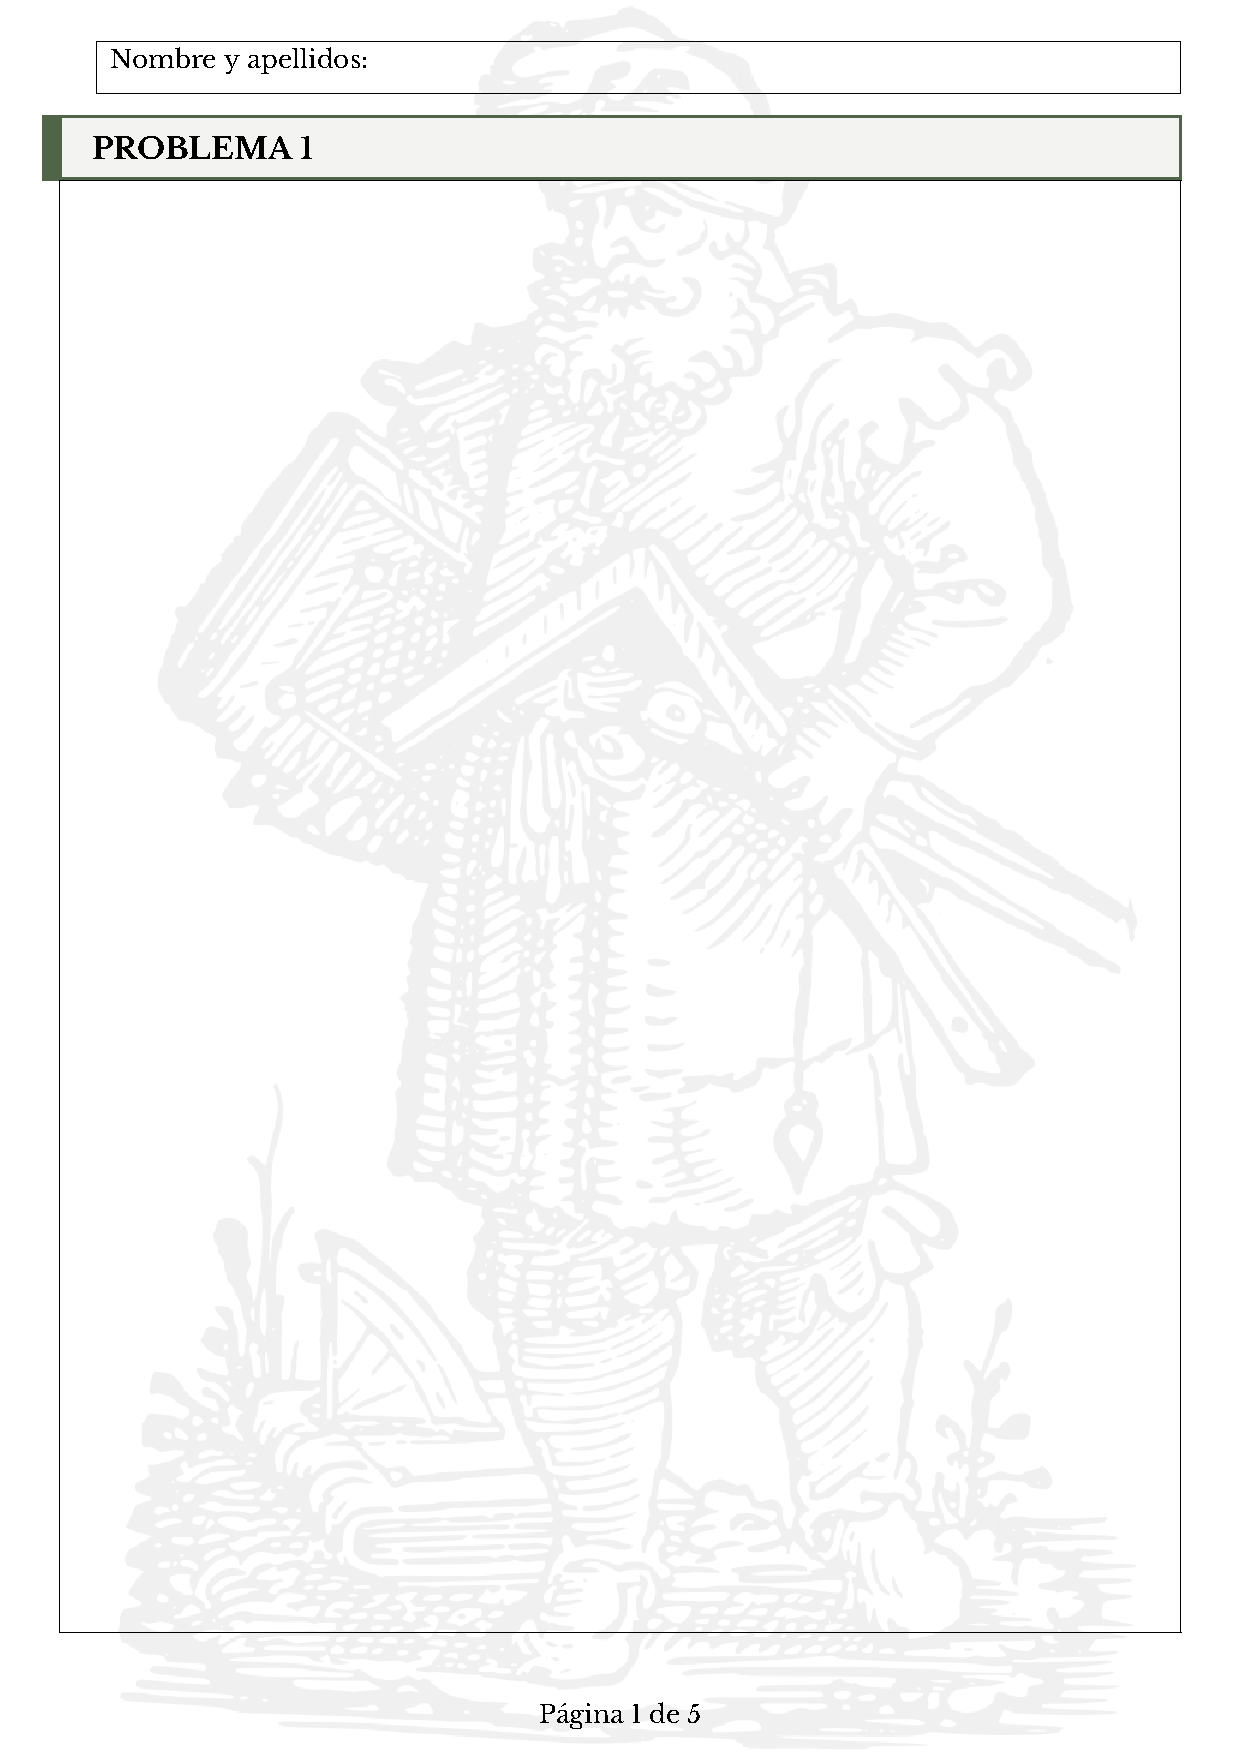
\includepdf[pages=-]{cuadernillo.pdf}

\end{document}